\documentclass[class=ctexart,crop=false]{standalone}

\usepackage{amsmath,amssymb,enumitem,empheq,tkz-euclide,
diagbox,wrapfig,pgfplots,geometry}
%\geometry{a4paper,scale=0.9}
\pgfplotsset{compat=newest}
%\usepgfplotslibrary{external}
%\tikzexternalize
\renewcommand\parallel{\mathrel{/\mskip-2.5mu/}}

\newcommand\px{\mathrel{/\mkern-5mu/}}  %平行
\newcommand\pxeq{\mathrel{\vcenter{     %平行且等于
\ialign{\hfil##\hfil\crcr
$\scriptstyle\px\!$\crcr
\noalign{\nointerlineskip\vskip1pt}$=$\crcr}}}}

%\setCJKmainfont{SimSun}       %设置西文字体为times new roman
%\setCJKsansfont{SimSun}             %设置中文字体为宋体
%\setCJKmonofont{STKaiti}
%\setsansfont{TeX Gyre Termes}            %设置typewriter family中文字体为楷体
%\setmonofont{TeX Gyre Termes}

\usetikzlibrary{calc,intersections,through,backgrounds,patterns}
\newcounter{para}
\newcommand\mypara{\par\refstepcounter{para}\thepara.\space}%设置typewriter family西文字体为times new roman
\newcommand*\circled[1]{\tikz[baseline=(char.base)]{
            \node[shape=circle,draw,inner sep=1pt] (char) {#1};}}

\newcommand{\rnum}[1]{\romannumeral #1}
\newcommand{\RNum}[1]{\uppercase\expandafter{\romannumeral #1\relax}}
\begin{document}
几何法:复杂不推荐\\
\begin{wrapfigure}{r}{0.3\textwidth}
    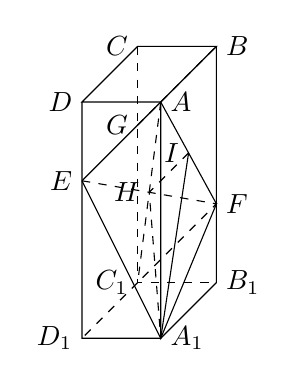
\begin{tikzpicture}[scale=1]
            \coordinate[label=right:$A_1$] (A_1) at (0,0);
            \coordinate[label=right:$A$] (A) at (0,3);
            \coordinate[label=right:$B_1$] (B_1) at ($sqrt(2)*(0.5,0.5)$);
            \coordinate[label=right:$B$] (B) at ($sqrt(2)*(0.5,0.5)+(0,3)$);
            \coordinate[label=left:$C_1$] (C_1) at ($sqrt(2)*(0.5,0.5)+(-1,0)$);
            \coordinate[label=left:$C$] (C) at ($sqrt(2)*(0.5,0.5)+(-1,3)$);
            \coordinate[label=left:$D_1$] (D_1) at (-1,0);
            \coordinate[label=left:$D$] (D) at (-1,3);
            \coordinate[label=left:$E$] (E) at (-1,2);
            \coordinate[label=right:$F$] (F) at ($sqrt(2)*(0.5,0.5)+(0,1)$);
            \coordinate[label=left:$H$] (H) at ($sqrt(2)*(0.25,0.25)+(-0.5,1.5)$);
            \coordinate[label=left:$G$] (G) at ($sqrt(2)*(0.5,0.5)+(-1,2)$);
            \coordinate[label=left:$I$] (I) at ($sqrt(2)*(0.25,0.25)+(0,2)$);
            \draw (A)--(B)--(C)--(D)--(A)--(A_1)--(B_1)--(B);
            \draw (I)--(A_1)--(D_1)--(D);
            \draw[dashed] (C)--(C_1)--(B_1);
            \draw[dashed] (C_1)--(D_1);
            \draw (E)--(A)--(F);
            \draw (E)--(A_1)--(F);
            \draw[dashed] (E)--(F)--(C_1);
            \draw[dashed] (G)--(B);
            \draw [dashed] (A)--(C_1);
            \draw [dashed] (I)--(H)--(A_1);
    \end{tikzpicture}
\end{wrapfigure}
\begin{enumerate}[label=(\arabic*)]
    \item 证明:\\
    连接 $C_1F$,取 $G$使 $C_1G=2CG$, 连接 $GB$ \\
    平面 $BCC_1B_1$内, $C_1G=\frac{2}{3}CC_1=\frac{2}{3}BB_1=FB\\$
    又$,FB \parallel C_1G$,则 $C_1GBF$ 为平行四边形\\
    则 $GB \pxeq C_1F $\\
    又 $CG=\frac{1}{3}CC_1=\frac{1}{3}DD_1=DE,DE \px CG$\\
    则 $ABGE$ 共面且为平行四边形,则 $GB \pxeq AE$ \\
    故 $AE \pxeq C_1F,AEC_1F$共面\\
    \item 解:\\
    记 $EF$ 中点为 $H$,由(1)知 $AEC_1F$ 为平行四边形\\  
    $C_1F=\sqrt{1+1}=\sqrt{2},AF=\sqrt{2^2+2^2}=2\sqrt{2},
    \\AC_1=\sqrt{1^2+2^2+3^2}=\sqrt{14},AH=HC_1=\frac{\sqrt{14}}{2}\\$
    由余弦定理:\\
    $\cos AHF=\frac{(\frac{\sqrt{14}}{2})^2+(\frac{EF}{2})^2-(2\sqrt{2})^2}{2\frac{\sqrt{14}}{2}\times \frac{EF}{2}}\\
    =-\cos C_1HF=-\frac{(\frac{\sqrt{14}}{2})^2+(\frac{EF}{2})^2-(\sqrt{2})^2}{2\frac{\sqrt{14}}{2}\times \frac{EF}{2}}$\\
    故有:  $ \begin{aligned}[t]
        \frac{7}{2}+\frac{1}{4}EF^2-8&=-\frac{7}{2}-\frac{1}{4}EF^2+2\\
            \frac{1}{2}EF^2&=2+8-7\\
        EF&=\sqrt{6}\\
    \end{aligned}$\\
    由 $AE^2+EF^2=2+6=8=AF^2$\\
    故 $\angle AEF=\frac{\pi}{2}$,即 $AE \perp EF$\\
    $\triangle A_1EF$中, 易知 $A_1F=A_1E=\sqrt{5}$\\
    故 $A_1H \perp EF$,作 $HI \px AE $交 $AF$ 于 $I$\\
    则 $\angle IHA_1$即为所求二面角的二面角\\
    易知 $HI$为 $\triangle FAE$中位线,$IH=\frac{1}{2}AE=\frac{\sqrt{2}}{2}$\\
    又 $H$为 $AC_1$中点,即立方体几何中心,故 $A_1H=\frac{1}{2}AC_1=\frac{\sqrt{14}}{2}$\\
    在平面 $AFA_1$中,通过辅助线易得 $A_1I=\sqrt{5}$\\
    $\triangle IHA_1$中, \\
    $\begin{aligned}[t]
        \cos \angle IHA_1&=\frac{(\frac{\sqrt{2}}{2})^2+(\frac{\sqrt{7}}{2})^2-(\sqrt{5})^2}{2\times \frac{\sqrt{2}}{2}\times \frac{\sqrt{14}}{2}}\\
        &=\frac{\frac{1}{2}+\frac{7}{2}-5}{\sqrt{7}}\\
        &=-\frac{\sqrt{7}}{7}\\
    \end{aligned}$\\
    故 $\sin IHA=\sqrt{1-(-\frac{\sqrt{7}}{7})^2}=\frac{\sqrt{42}}{7}$\\
    故二面角 $A-EF-A_1$的正弦值为 $\frac{\sqrt{42}}{7}$\\
\end{enumerate}
\end{document}